

\section{Graphical User Interface} \label{GUI}

%There are two different graphical user interfaces available for
%\freefempp:

%\begin{itemize}
%\item 
\texttt{FreeFem++-cs} is part of the standard \freefempp
package. It runs on Linux, MacOS X and Windows.
%\item \texttt{FFedit} is available as a separate package. It runs on
%Linux and MacOS~X and requires tcl/tk to be installed.
%\end{itemize}

%\subsection{FreeFem++-cs}

``-cs'' stands for ``client/server''. The executable program named
\texttt{FreeFem++-cs} contains code for running a graphical user
interface client and a computational server. The server is
automatically started every time every time the user asks for a script
to be run. To run \texttt{FreeFem++-cs}, just type its name in,
optionally followed by a script name. It will open a window
corresponding to fig. \ref{fig:FreeFem++-cs}.

\begin{figure}[htbp]
\begin{center}
  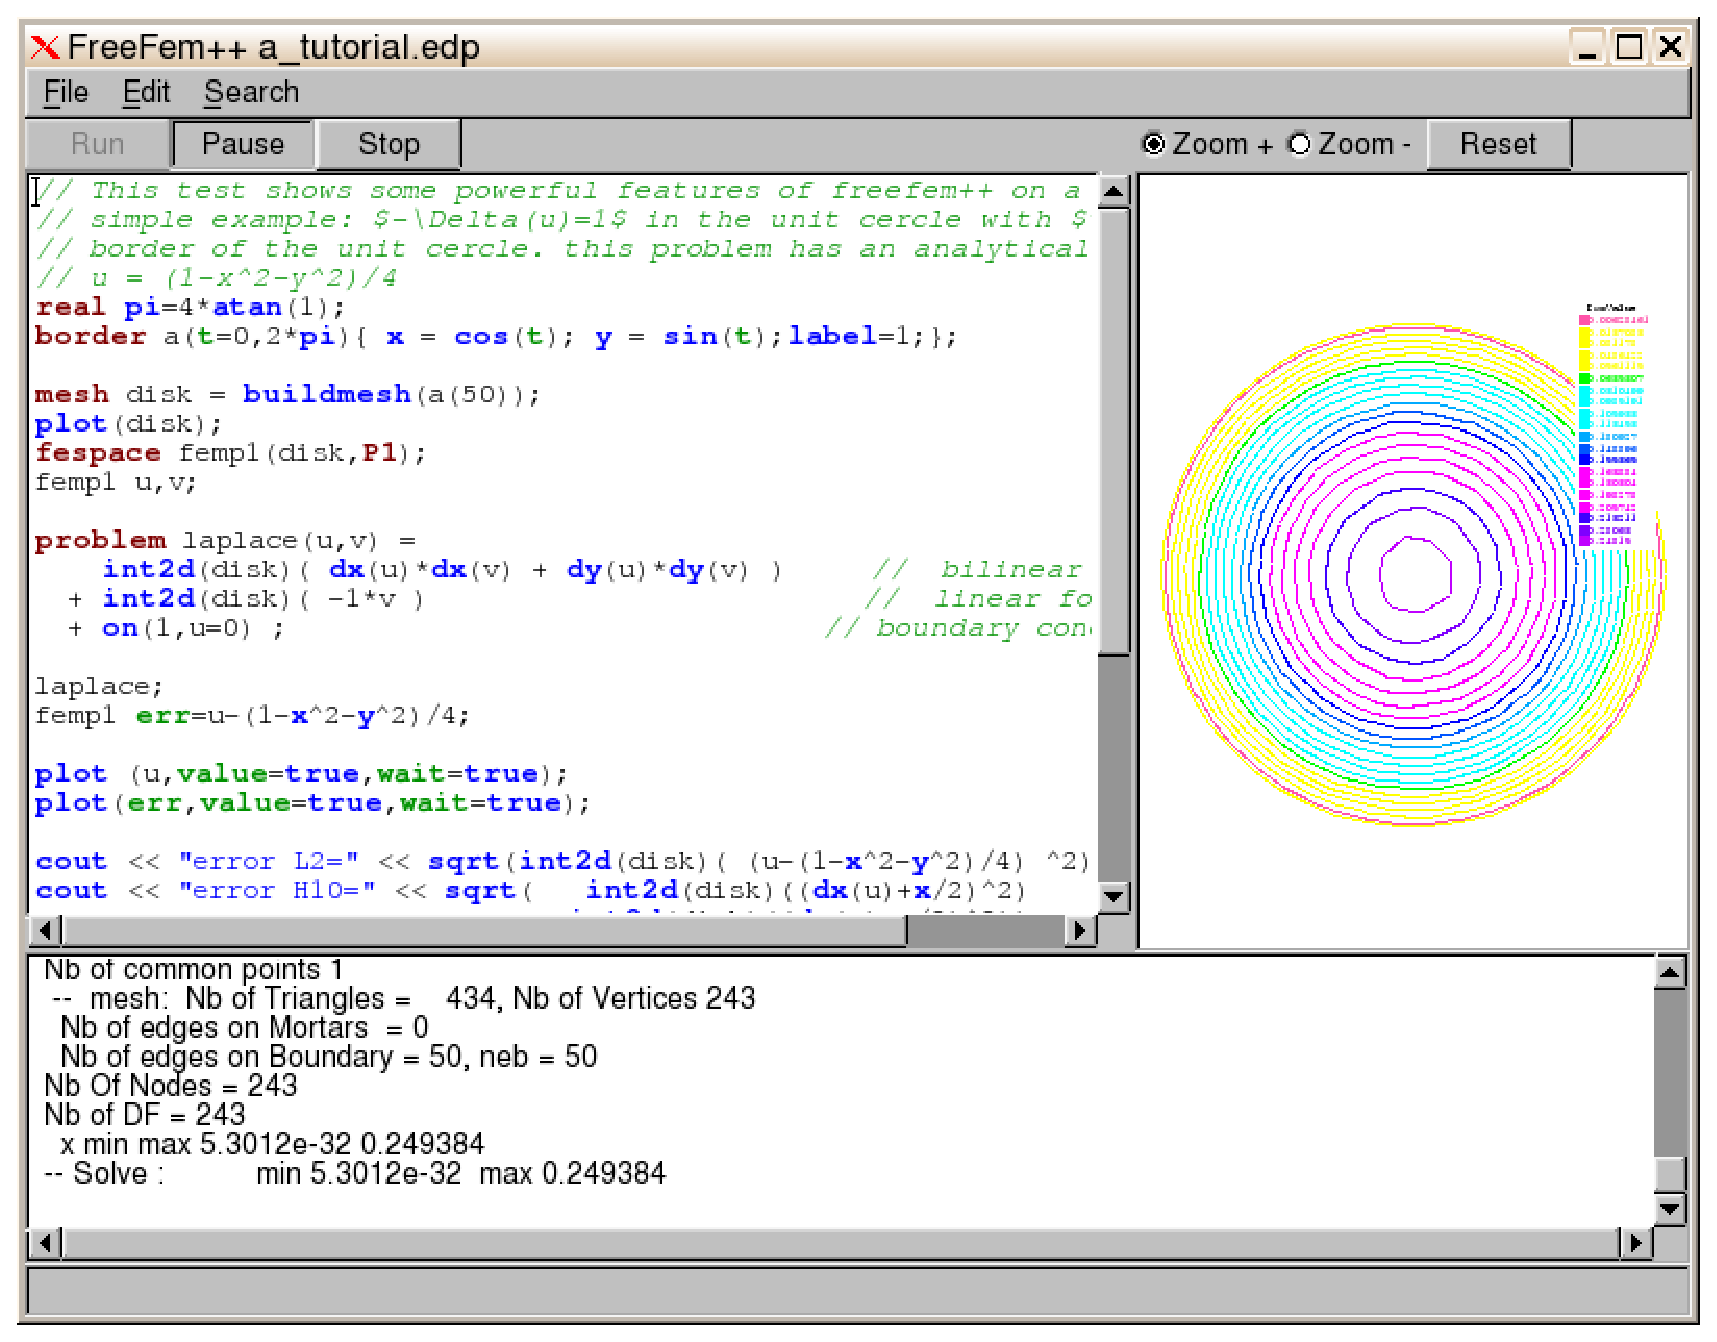
\includegraphics[height=10cm]{FreeFem++-cs}
\end{center}
  \caption{\texttt{FreeFem++-cs} main window}
  \label{fig:FreeFem++-cs} \index{label}
\end{figure}

\bigskip

The main characteristics of \texttt{FreeFem++-cs} are~:

\begin{itemize}
\item A main window composed of three panels~: editor with syntax
highlighting (right), \freefempp messages (bottom) and graphics
(left).
\item Panel sizes can be changed by dragging their borders with the
mouse. Any of the three panels can be made to fill the whole window.
\item The edited script can be run at any time by clicking on the
``Run'' button.
\item Dragging a \freefempp script file icon from a file manager into
the editor window makes \texttt{FreeFem++-cs} edit that script.
\item Graphics can be examined (e.g. zoomed) while \freefempp is
running.
\item A running \freefempp computation can be paused or stopped at any
time.
\end{itemize}

\bigskip

All commands should be self-explanatory. Here are just a few
useful hints~:

\begin{itemize}
\item There is no need to save a \freefempp script to run it. It is
  run exactly as displayed in the editor window, and the corresponding
  file is not touched.
\item The current directory is updated every time a script is loaded
  or saved. All \texttt{include} directives are therefore relative to
  the directory where the main script is located.
\item Specifying \texttt{wait=1} in a \texttt{plot} command is exactly
  equivalent to clicking on the ``Pause'' button when the plot is
  displayed.
\item In zoom mode, if your mouse has more than one button, a
  middle-click resets any zooming coefficient, and a right-click zooms
  in the opposite way of the left-click.
\end{itemize}

%\subsection{FFedit}

%FFedit runs on Linux and MacOSX.

%\subsubsection{Installation of Tcl and Tk}

%You have to install tcl8.4.6 and tk8.4.6 for the GUI to work.\\
%First go to http:\\
%//www.tcl.tk./software/tcltk/downloadnow84.tml \\
%and download :\\
%tcl8.4.6-src.tar.gz and tk8.4.6-src.tar.gz\\
%Then do :\\
%tar zxvf tcl8.4.6-src.tar.gz\\
%tar zxvf tk8.4.6-src.tar.gz\\
%It creates two directories : tcl8.4.6 and tk8.4.6\\
%Now do : \\
%cd tcl8.4.6\\
%cd unix (if your OS is Linux or MacOSX)\\
%./configure\\
%make\\
%make install\\
%\\
%then \\
%cd tk8.4.6\\
%cd unix\\
%./configure\\
%make\\
%make install\\
%\\
%At the end of installation, you have to find where is your binary ``wish'' or ``wish84'' or ``wish8.4'' by typing :\\
%-$>$ which wish (or wish84 or wish8.4)\\
%If wish84 does exist it is all. If not, you have to go in the directory where is ``wish'' or ``wish8.4'' (for example /usr/bin/)\\
%and then create a link :\\
%-$>$ ln -s wish wish84\\
%or\\
%-$>$ ln -s wish8.4 wish84\\

%\subsubsection{Description}

%The Graphic User Interface is in the directory called FFedit.
%You can run it by typing ./FFedit.tcl\\
%\
%The Graphic User Interface shows a text window with buttons on the left and right side, a horizontal menu bar above and an entry below where you can see the path of the script when it is opened or where you can type the path of a script to run it.\\
%\\
%This is the description of the different functions of the GUI :\\
%\\
%*New : you can access it by the button ``New'' on the right side or by selecting it in the menu File on the horizontal bar.\
%It deletes the current script and enables you to type a new script.\\
%\\
%*Open : you can access it by the button ``Open'' on the right side or by selecting it in the menu File or by typing simultaneously ctrl+o on the keyboard.\
%It enables you to select a script which has been saved. This script is then opened in the text window. Then, you can modify it, save the changes, save under another name or run it.\\
%\\
%*Save : you can access it by the button ``Save'' on the right side or by selecting it in the menu File or by typing simultaneously ctrl+s on the keyboard.\
%It enables you to save the changes of a script.\\
%\\
%*Save as : you can access it by the button ``Save As'' on the right side or by selecting it in the menu File.\\
%It enables you to locate where you want to save your script and to choose your the name of your script.\\
%\\
%*Run : you can access it by the button ``Run'' on the right side or by selecting it in the menu File or by typing simultaneously ctrl+r on the keyboard.\\
%It enables you to run the current script.\\
%Warning: when you run by typing ctrl+r, the cursor must be in the text window.\\
%\\
%*Print : you can access it by the button ``Print'' on the right side or by selecting it in the menu File or by typing simultaneously ctrl+p on the keyboard.\\
%It enables you to print your script. You have to choose the name of the printer.\\
%\\
%*Help (under construction) : you can access it by the button ``Help'' on the left side. When an example is opened, it shows you a documentation about this example.\\
%Warning : The bottom of each page is not accessible, you have to print to see the entire document.\\
%\\
%*Example : you can access it by the button ``Ex'' on the left side.\
%It runs a little example.\\
%\\
%*Read Mesh : you can access it by the button ``R.M'' on the left side.\
%It enables you to read a mesh which has been saved. It adds the command in your script so that you can use it in your script.\\
%\\
%*Polygonal Border : you can access it by the button ``P.B'' on the left side.\\
%It enables you to build a polygonal border.\\
%When you click on this button, a new window is opened : you have to click on the button ``Border'' then it asks you how many borders you want. When you enter a number and click on ``OK'' the exact number of couple of entries enable you to enter the coordinates of the vertices. And then you have to enter the number of points on each border. The border number 1 is the segment between the vertex number 1 and the vertex number 2 ...etc...\\
%You must turn in the opposite sens of needles of a watch.\\
%When you have finished, you have to click on the button ``Build''. It builds the domain with polygonal border and shows the result.\\
%Then you can save the result by clicking on the button ``S.Mesh''. Choose the extension .msh for the name.\\
%\\
%*Navier Stokes : you can access it by the button ``N.S'' on the left side.\\
%A new window is opened. You have to build your polygonal domain by clicking on the button ``Border'' it works like the Polygonal Border function.\\
%You can save by clicking on the button ``S.Mesh''. Choose the extension .msh for the name.\\
%Then you have to choose the Limits Condition by clicking on the buton ``L.C''.\\
%First choose between ``Free'' or ``Imposed', then click on the button ``Validate'' and enter the expression of Imposed condition. You have to enter the tangential and the normal component of the velocity. Then click on ``Validate'' again.\\
%The expression of the limit condition can be a number but a mathematical expression as well.\\
%\\
%*emc2 : you can access it by the button ``emc2''. It runs emc2 the mesh building software \\
%(http://www-rocq1.inria.fr/gamma/cdrom/\\
%www/emc2/fra.htm)\\
%\\
%*Set up : you can access it by the button ``set up''. It is the first thing you have to do when you use FFedit for the first time.\\
%When you click on this button, a new window is opened, with two entries where you have to enter the path of the binary of FreeFem++ (where you compiled or installed) and the path of the scripts (programs written with FreeFem++) for instance the examples provided in FreeFem++.\\
%\\
%*Undo : you can access it by selecting in the menu Edit or by typing simultaneously ctrl+z. It is an unlimited undo function.\\
%\\
%*Redo : you can access it by selecting in the menu Edit or by typing simultaneously ctrl+e. It is an unlimited redo function.\\
%\\
%*Cut : you can access it by selecting in the menu Edit or by typing simultaneously ctrl+x on the keyboard.\\
%\\
%*Copy : you can access it by selecting in the menu Edit or by typing simultaneously ctrl+c on the keyboard.\\
%\\
%*Paste : you can access it by selectiog in the menu Edit or by typing simultaneously ctrl+y on the keyboard.\\
%\\
%*Delete : you can access it by selecting in the Edit menu. It is a Delete function.\\
%\\
%*Select all : you can access it by selecting in the Edit menu or by typing simultaneously ctrl+l. This function select all the text you have written, so you can delete, cut copy paste etc...\\
%\\
%*Background : you can access it by selecting in the menu Color. You can then choose the color of the background.\\
%\\
%*Foreground : you can access it by selecting in the menu Color. You can then choose the color of the foreground.\\
%\\
%*Syntax Color : you can access it by selecting in the menu Color. It enables the syntax coloring of your FreeFem++ script.\\
%\\
%*Family : you can access it by selecting in the menu Font. You can then choose the style of your characters.\\
%\\
%*Size : you can access it by selecting in the menu Font. You can then choose the size of your characters.\\
%\\
%*Find : you can access it by selecting in the menu Search. It enables you to find a word in the whole text. (This function doesn't work yet.)\\
%\\
%*Find next : you can access it by slecting in the menu Search. It enables you to find a word from the position of the cursor.(This function doesn't work yet.)\\
%\\
%*Replace : you can access it by selecting in the menu Search. It enables you to replace a word by another in the whole text.\\

%\subsubsection{Cygwin version}

%This version is for Windows.\\

%\subsubsection{Installation of Cygwin}
%First you have to go to the site:\\
%http://www.cygwin.com \\
%Click on ``Install or Update now''\\
%A window appears. \\
%Click on ``Open'' then ``Next'' and then choose ``Install from Internet''\\
%Click on ``Next'' twice and choose ``Direct Connection''.\\
%Then choose one of the download sites.\\
%For instance : ftp://ftp-stud.fht-esslingen.de\\
%Then choose in each category the options to install. \\
%(click on the symbol + for each, you can then see the options appear)\\
%\\
%Here are the required options for FreeFem++ and TCL TK to work :\\
%+ all options of ``Devel'' (it includes gcc ...etc...)\\
%+ all options of ``Graphics'' (specially ``Gnuplot'' to be able \\
%to see the results of FreeFem++ on a graphic)\\
%+ all options of X11 and XFree86 \\
%\\
%You can install ``Xemacs'' and others editors in the category ``Editors''.\\
%\\
%Then click on ``Next'' and wait that Cygwin is installed.\\
%Then an ic�ne appears on yours Desktop.\\
%Click on it and the Cygwin window is opened. It is like an Unix terminal.\\
%\\
%To work on a terminal X type : \\
%-$>$ startX\\
%You will have to work on a terminal X to have Gnuplot and visualize \\
%the results of FreeFem++ scripts)\\
%\\
%Now you have to compile and install FreeFem++.\\
%\\
%\subsubsection{Compilation and Installation of FreeFem++ under Cygwin}
%go to the site :\\
%http://www.freefem.org\\
%click on FreeFem++\\
%and download FreeFem++ (the version when I wrote this is 1.38)\\
%Choose to download in your cygwin/home/you directory.\\
%\\
%Then on your terminal Cygwin type :\\
%-$>$ tar zxvf freefem++.tgz\\
%to uncompress this file.\\
%\\
%Go into FreeFem++v1.38 directory by typing:\\
%-$>$ cd FreeFem++v1.38\\
%\\
%Now you have to compile FreeFem++.\\
%type:\\
%-$>$ make all HOSTTYPE=i-386\\
%to compile FreeFem++\\
%If there is an error : ``... -ldl : no such file or directory''\\
%Then you have to modify the Makefile-i386 which is in the directory src:\\
%-$>$ cd src \\
%Edit it (with xemacs for example):\\
%-$>$ xemacs Makefile-i386\\
%at line 1 : replace ``LIBLOCAL = -ldl'' by ``\#LIBLOCAL = -ldl''\\
%It will comment this line because -ldl is not on your machine.\\
%Then return to the main directory\\
%-$>$ cd\\
%and type:\\
%-$>$ make all HOSTTYPE=i-386\\
%\\
%At the end of compilation, a directory called ``c-i386'' is created.\\
%In this directory you can find the binary FreeFem++.\\
%\\
%You can now run an example:\\
%First open an X terminal:\\
%-$>$ startX\\
%In this terminal go in to FreeFem++v1.38:\\
%-$>$ cd FreeFem++v1.38\\
%and type:\\
%-$>$c-i386/FreeFem++ examples++-tutorial/adapt.edp\\
%You can then see the gnuplot window with the graphical results.\\
%\\

%\subsubsection{Compilation and Installation of tcl8.4.0 and  tk8.4.0 under Cygwin}
%Now if you want to use the Graphical User Interface of FreeFem++\\
%(called FFedit)\\
%you have to install the language TCL TK in which FFedit has been written.\\
%The version which works under cygwin is tcl8.4.0 and tk8.4.0\\
%The latest version when I wrote this is tcl8.4.6 and tk8.4.6\\
%\\
%DON'T USE IT \\
%\\
%It works under Linux and MacOsX but not under Cygwin.\\
%\\
%You have to download tcl8.4.0 and tk8.4.0 :\\
%For instance, go to Google.fr and type download tcl tk 8.4.0\\
%And choose the ``Sourceforge.net: Project Filelist''.\\
%Choose :\\
%tcl8.4.0-src.tar.gz and tk8.4.0-src.tar.gz\\
%When the download is finished you have to uncompress these directories:\\
%-$>$ tar zxvf tcl8.4.0-src.tar.gz\\
%-$>$ tar zxvf tk8.4.0-src.tar.gz\\
%\\
%\\
%tcl8.4.0 and tk8.4.0 will work under Cygwin only if you apply \\
%a patch on both:\\
%These patches are on the site:\\
%http://www.xraylith.wisc.edu/~khan/software/tcl\\
%Choose ``Tcl/Tk8.4.0 for Cygwin\\
%Click on ``very preliminary Cygwin ports of Tcl/Tk8.4.0\\
%You are then on the site ftp\\
%Follow the instructions of the README or follow these instructions:\\
%\\
%1) Run :\\
%-$>$ xemacs tcl-8.4.0-cygwin.diff\\
%By doing this, you create a new file called ``tcl-8.4.0-cygwin.diff''\\
%on the site ftp click on ``tcl-8.4.0-cygwin.diff''\\
%Do a Copy/Paste of the contain into your xemacs window and save it.\\
%\\
%2) Do the same with ``tk-8.4.0-cygwin.diff''\\
%\\
%Now you have to apply the patch in tcl8.4.0 and tk8.4.0\\
%The two previous patch files (.diff) must be respectively \\
%in tcl8.4.0 and tk8.4.0 directories.\\
%-$>$ cp tcl-8.4.0-cygwin.diff tcl8.4.0\\
%-$>$ cp tcl-8.4.0-cygwin.diff tk8.4.0\\
%(If the two files are one level under tcl8.4.0 and tk8.4.0)\\
%\\
%Now apply the patches:\\
%type:\\
%\\
%-$>$ cd tcl8.4.0\\
%-$>$ patch -p0 -s $<$ tcl-8.4.0-cygwin.diff\\
%\\
%-$>$ cd
%\\
%-$>$ cd tk8.4.0\\
%-$>$ patch -p0 -s $<$ tk-8.4.0-cygwin.diff\\
%\\
%Now you can compile and install TCL TK under Cygwin:\\
%\\

%
%* compilation and installation of tcl8.4.0\\
%\\
%Go in to the directory tcl8.4.0/win\\
%-$>$ cd tcl8.4.0\\
%-$>$ cd win\\
%Then type :\\
%-$>$ ./configure\\
%The two steps remaining are make and make install\\
%type\\
%-$>$ make\\
%The compilation starts, when finished install by typing:\\
%-$>$ make install\\
%\\
%When finished try to see if it works by typing:\\
%-$>$ tclsh84\\
%if ok quit by typing ctrl-c\\

%*Compilation and installation of tk8.4.0\\
%\\
%Go in to the directory tk8.4.0/win\\
%-$>$ cd tk8.4.0\\
%-$>$ cd win\\
%Then type :\\
%-$>$ ./configure\\
%The two steps remaining are make and make install\\
%type\\
%-$>$ make\\
%The compilation starts, if you have errors like :\\
%\\
%windres -o tk.res.o --include ``C:/cygwin/home/ly/tk8.4.0/generic'' \\
%--include ``C Option-I is deprecated for setting the input format,\\
% please use -J instead''\\
%windres : can't open icon file 'tk.ico' : no such file or directory\\
%\\
%This file 'tk.ico' is in fact in the directory win/rc\\
%You have to copy it in the directory 'generic':\\
%Be in tk8.4.0\\
%type :\\
%-$>$ cp win/rc/tk.ico generic/\\
%\\
%If you compile again you will see that there is the same \\
%errors with the files:\\
%``buttons.bmp'' ``cursor00.cur'' ``cursor02.cur'' ...etc... \\
%``wish.exe.manifest'' and ``wish.ico''\\
%\\
%Do the same for these files.\\
%For the cursor*.cur files do once the command:\\
%-$>$ cp win/rc/cursor*.cur generic/\\
%\\
%when finished install by typing:\\
%-$>$ make install\\
%\\
%When finished try to see if it works by typing:\\
%-$>$ wish84\\
%if ok quit by typing ctrl-c\\

%\subsubsection{Use}
%Now everything is ok to use FFedit and FreeFem++ under Windows by Cygwin.\\
%WARNING: if you work on the Cygwin terminal you will not be able \\
%to see the graphical results of FreeFem++.\\
%\\
%You have to run an X terminal and run FFedit under this X terminal:\\
%\\
%To run an X terminal under cygwin type on your Cygwin terminal:\\
%-$>$ startX\\
%\\
%An X terminal runs:\\
%Under this terminal:\\
%type\\
%-$>$ cd FFedit\\
%-$>$ ./FFedit.tcl\\

